\section{Entwurf}
In diesem Kapitel stellen kurz die Plattformen vor auf die wir uns bei der Entwicklung beschränken wollen. Anschließend unser System mithilfe eines Diagramms grundlegend vor. Im letzten Abschnitt gehen wir auf die wichtigsten Aspekte beim Design der Smartwatch-Anwendung ein.

\subsection{Plattformen}
In diesem Projekt geht es im Wesentlichen um zwei Aspekte: Zum einen wollen wir uns mit der Anwendungsentwicklung auf Smartwatches beschäftigen, zum anderen wollen wir einen neuen Ansatz zur Lokalisation in Gebäuden ausprobieren. Aus diesem Grund verzichten wir auf aufwendige hybride Lösungen und beschränken uns auf die Entwicklung zweier nativer Applikationen für die Android- bzw. Android-Wear-Plattform. Für die Lokalisation innerhalb des Gebäudes wollen wir Bluetooth-Beacons einsetzten. Bezüglich der Beacons haben wir uns, vor allem aufgrund des niedrigen Stromverbrauchs, auf den Standard Bluetooth LE festgelegt.

\subsection{Systemübersicht}
\label{sec:systemuebersicht}
Abbildung \ref{fig:Übersicht} zeigt eine grundlegende Übersicht unseres Systems:

\begin{figure}[H]
\centering
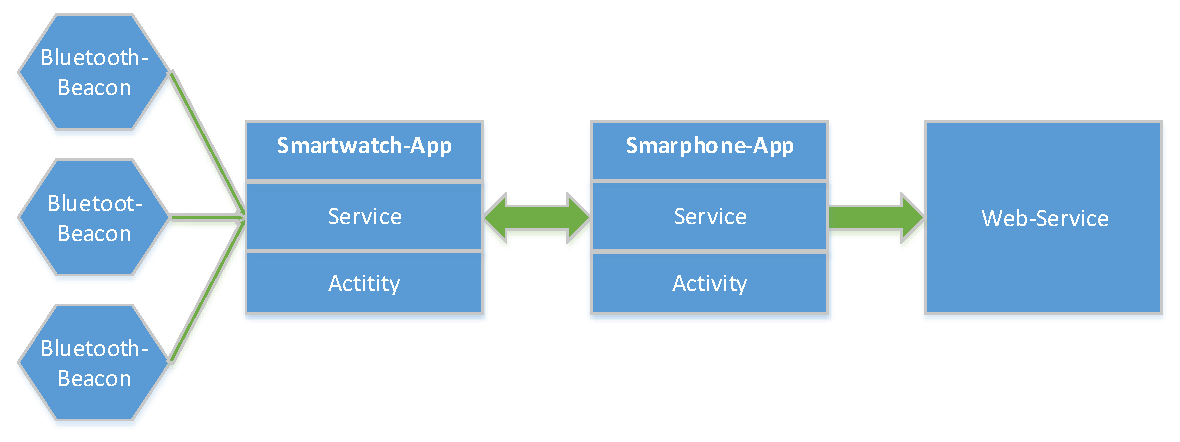
\includegraphics[width=0.95\linewidth]{Bilder/Uebersicht}
\caption{Systemübersicht}
\label{fig:Übersicht}
\end{figure}

Im ersten Schritt, noch vor Inbetriebnahme unseres Systems, müssen die Räume des Gebäudes mit Bluetooth-Beacons bestückt werden. Diese senden kontinuierlich ein Signal, dass durch die Smartwatch-App empfangen wird. Bei der Inbetriebnahme des Systems muss zunächst jeder Raum des Gebäudes ausgemessen werden. Ein entsprechender Scan lässt sich über die Smartphone-App durchführen. Nachdem das Gebäude vollständig vermessen wurde, muss im nächsten Schritt das mathematische Modell, dass zur Erkennung des aktuellen Raumes benötigt wird, berechnet werden. Da diese Berechnung in einen Webservice ausgelagert ist, wird an dieser Stelle einmalig eine Internetverbindung vorausgesetzt. Nach erfolgreicher Berechnung ist das System betriebsbereit und erkennt von nun an automatisch dass Betreten bzw. Verlassen eines Raumes.

Nachdem das System initial eingerichtet wurde, benötigt der Anwender sein Smartphone nur noch, um Notizen im aktuellen Raum zu hinterlegen. Über die Smartphone-App lassen sich Notizen zusätzlich mit den Ereignissen Verlassen oder Betreten des Raumes verknüpfen. Die Daten werden nach der Eingabe an die Smartwatch geschickt und dort gespeichert. Damit wird das Smartphone für den aktiven Systembetrieb nicht mehr benötigt.

%\subsection{Design}
% Hier auf Usability und Design der Smartwatch-App einzugehen macht keinen Sinn, da wir dafür ein eigenes Kapitel haben!


